\chapter{The Chain}
\chapter{Proof-of-Work \small{\textsf{DRAFT}}}\label{chapter:pow}

In the last chapter, we discussed the necessity for blocks as a mechanism to enforce \emph{periods of silence} so that double spends
can be adequately separated in time.  We then linked blocks together into chains in order to ensure freshness so that an adversary cannot
retroactively bring blocks mined and withheld in the old past. However, we left the notion of ``freshness'' and block validation
undefined. In this chapter, we will fill in all the missing details of how blocks and chains are verified. By the end of this chapter,
we will have a rudimentary, yet complete and secure, blockchain protocol.

\section{The Target}

Previously, we designed the proof-of-work inequality $H(B) \leq T$ in order to create \emph{rare events} and \emph{periods of silence}
as a moderately hard version of the exponentially hard hash preimage problem. In order to prevent double spends, we needed to ensure
that blocks are spaced $\Delta$ apart. Let us now calculate the correct value of $T$ so that block production is spaced more than
$\Delta$ time apart. To do this, we need to first find out when the proof-of-work inequality holds. If we start
with a freshly generated $\ctr$ and place it into $B = s \conc \overline{x} \conc \ctr$, what is the probability that $H(B) \leq T$?
This question is not straightforward to answer, because the output of a hash function may not be uniformly distributed (see also
Problem~\ref{problem:small-hash}).

\section{The Stochastic Nature of Work}

\section{Freshness}
Freshness provides an arrow of time. Since each new block includes the hash of the previous block we can confidently say that the new block was produced after the previous block. This prevents adversaries from premining blocks and adding them when convenient because the adversary must include the hash of the previous block when producing the block that comes after that.
% In other words, proof-of-work combined with chaining gives an \textit{arrow of time}.

This makes it impossible to go back and change a block without having to change all the blocks that came after that block as shown in Figure~\ref{fig:Blockchain}.

\begin{figure}[H]
	\centering
\tikzset{every picture/.style={line width=0.75pt}} %set default line width to 0.75pt

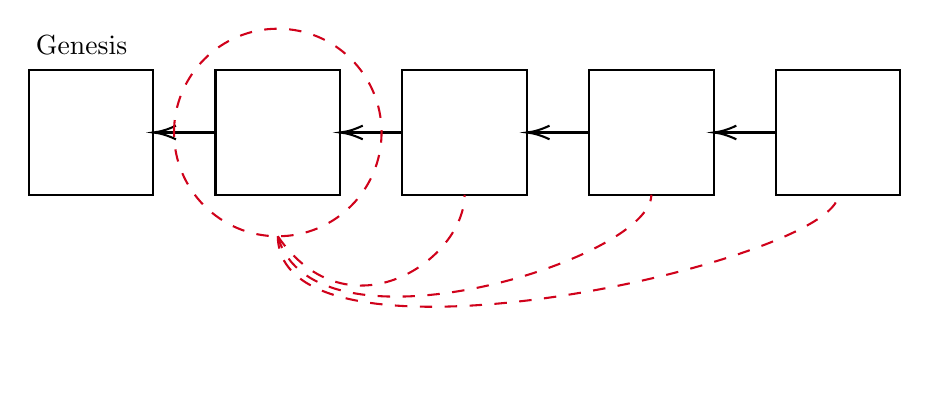
\begin{tikzpicture}[x=0.75pt,y=0.75pt,yscale=-1,xscale=1]
%uncomment if require: \path (0,152); %set diagram left start at 0, and has height of 152

%Shape: Square [id:dp23344059832601505]
\draw   (20,30) -- (80,30) -- (80,90) -- (20,90) -- cycle ;
%Straight Lines [id:da7766615176026717]
\draw    (110,60) -- (82,60) ;
\draw [shift={(80,60)}, rotate = 360] [color={rgb, 255:red, 0; green, 0; blue, 0 }  ][line width=0.75]    (10.93,-3.29) .. controls (6.95,-1.4) and (3.31,-0.3) .. (0,0) .. controls (3.31,0.3) and (6.95,1.4) .. (10.93,3.29)   ;
%Shape: Square [id:dp7147823925662169]
\draw   (110,30) -- (170,30) -- (170,90) -- (110,90) -- cycle ;
%Straight Lines [id:da007438116619583823]
\draw    (200,60) -- (172,60) ;
\draw [shift={(170,60)}, rotate = 360] [color={rgb, 255:red, 0; green, 0; blue, 0 }  ][line width=0.75]    (10.93,-3.29) .. controls (6.95,-1.4) and (3.31,-0.3) .. (0,0) .. controls (3.31,0.3) and (6.95,1.4) .. (10.93,3.29)   ;
%Shape: Square [id:dp9572022268983138]
\draw   (200,30) -- (260,30) -- (260,90) -- (200,90) -- cycle ;
%Straight Lines [id:da6716771568739017]
\draw    (290,60) -- (262,60) ;
\draw [shift={(260,60)}, rotate = 360] [color={rgb, 255:red, 0; green, 0; blue, 0 }  ][line width=0.75]    (10.93,-3.29) .. controls (6.95,-1.4) and (3.31,-0.3) .. (0,0) .. controls (3.31,0.3) and (6.95,1.4) .. (10.93,3.29)   ;
%Shape: Square [id:dp03760878338773743]
\draw   (290,30) -- (350,30) -- (350,90) -- (290,90) -- cycle ;
%Straight Lines [id:da18396718235576381]
\draw    (380,60) -- (352,60) ;
\draw [shift={(350,60)}, rotate = 360] [color={rgb, 255:red, 0; green, 0; blue, 0 }  ][line width=0.75]    (10.93,-3.29) .. controls (6.95,-1.4) and (3.31,-0.3) .. (0,0) .. controls (3.31,0.3) and (6.95,1.4) .. (10.93,3.29)   ;
%Shape: Square [id:dp872209963300697]
\draw   (380,30) -- (440,30) -- (440,90) -- (380,90) -- cycle ;
%Shape: Ellipse [id:dp04492348308330163]
\draw  [color={rgb, 255:red, 208; green, 2; blue, 27 }  ,draw opacity=1 ][dash pattern={on 4.5pt off 4.5pt}] (90,60) .. controls (90,32.39) and (112.39,10) .. (140,10) .. controls (167.61,10) and (190,32.39) .. (190,60) .. controls (190,87.61) and (167.61,110) .. (140,110) .. controls (112.39,110) and (90,87.61) .. (90,60) -- cycle ;
%Curve Lines [id:da5130772526447398]
\draw [color={rgb, 255:red, 208; green, 2; blue, 27 }  ,draw opacity=1 ] [dash pattern={on 4.5pt off 4.5pt}]  (140,110) .. controls (174,159.35) and (230,121.35) .. (230,90) ;
%Curve Lines [id:da8040106292717784]
\draw [color={rgb, 255:red, 208; green, 2; blue, 27 }  ,draw opacity=1 ] [dash pattern={on 4.5pt off 4.5pt}]  (140,110) .. controls (157,171.35) and (320,121.35) .. (320,90) ;
%Curve Lines [id:da6486701606800711]
\draw [color={rgb, 255:red, 208; green, 2; blue, 27 }  ,draw opacity=1 ] [dash pattern={on 4.5pt off 4.5pt}]  (140,110) .. controls (141,182.35) and (410,121.35) .. (410,90) ;

% Text Node
\draw (22,12) node [anchor=north west][inner sep=0.75pt]   [align=left] {Genesis};


\end{tikzpicture}
	\caption{Chaining blocks prevents changing the old blocks as this would invalidate the proof-of-work equation for the blocks following it in the chain.}
	\label{fig:Blockchain}  %Tag for referring to figure in text.
\end{figure}

\section{Determining the Target Parameter}
For simplicity, consider that $B$ is randomly chosen in $\{0,1\}^\kappa$. Then,
\begin{equation}
    \Pr[H(B) \leq T] = {\frac{T}{2^\kappa}} = p
\end{equation}
\begin{itemize}
\item $p$: Probability of successful query
\item $q$: hash power of a single party
\item $n$: number of parties participating in network
\end{itemize}

Here, we think of one party as one unit of computation. All parties in the network are simultaneously trying to create a block.

The target variable $T$ should be chosen such that the time taken to generate a valid nonce ($B$) should be greater than the network delay.

\begin{equation}
    \frac{1}{pnq} = \Delta
\end{equation}
where $\Delta$ is the network delay.

\begin{equation}
    T = \frac{2^\kappa}{\Delta nq}
\end{equation}

Here, $qn$ is the total hashing power of the network. We can see that as $qn$ increases T should decrease. This means that it should become harder for each party to generate a valid nonce.
Increasing the network delay will also similarly require $T$ to be decreased.

\section{Accounting for Stochastic Nature of Proof of Work}

Ideally we would want that all blocks are produced with the same delay as decided by the equation above. However, the Proof-of-Work algorithm is stochastic. Thus based on our above calculation, the expected time to produce a block will be $\Delta$ but in practice there may be instances where blocks are produced in quick succession without the required time delay. This takes us back to square one in terms of thinking about how to prevent double spends. Figure~\ref{fig:Convergence events} shows convergence opportunities (i.e. periods of time where an event happened spaced out by more than $\Delta$ from both the previous and next event) and conflicting events (i.e. periods of time where two events happened in a time interval shorter than $\Delta$) produced during the mining process.

\begin{figure}[H]
\centering
\tikzset{every picture/.style={line width=0.75pt}} %set default line width to 0.75pt

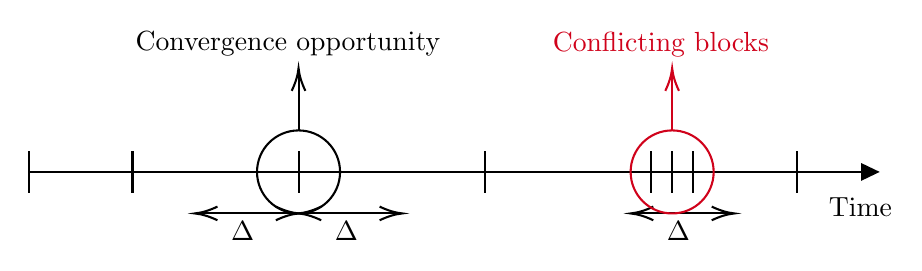
\begin{tikzpicture}[x=0.75pt,y=0.75pt,yscale=-1,xscale=1]
%uncomment if require: \path (0,132); %set diagram left start at 0, and has height of 132

%Straight Lines [id:da23525023892191266]
\draw    (140,81) -- (547,81) ;
\draw [shift={(550,81)}, rotate = 180] [fill={rgb, 255:red, 0; green, 0; blue, 0 }  ][line width=0.08]  [draw opacity=0] (8.93,-4.29) -- (0,0) -- (8.93,4.29) -- cycle    ;
%Straight Lines [id:da7960445132740581]
\draw    (140,71) -- (140,91) ;
%Straight Lines [id:da29783337527097675]
\draw    (270,71) -- (270,91) ;
%Straight Lines [id:da33677894078119586]
\draw    (190,71) -- (190,91) ;
%Straight Lines [id:da5399367214918731]
\draw    (360,71) -- (360,91) ;
%Straight Lines [id:da09675758542474289]
\draw    (440,71) -- (440,91) ;
%Straight Lines [id:da5769918595193868]
\draw    (450,71) -- (450,91) ;
%Straight Lines [id:da31319754434895075]
\draw    (460,71) -- (460,91) ;
%Straight Lines [id:da33141985537928864]
\draw    (510,71) -- (510,91) ;
%Shape: Ellipse [id:dp7733367297760827]
\draw   (250,81) .. controls (250,69.95) and (258.95,61) .. (270,61) .. controls (281.05,61) and (290,69.95) .. (290,81) .. controls (290,92.05) and (281.05,101) .. (270,101) .. controls (258.95,101) and (250,92.05) .. (250,81) -- cycle ;
%Straight Lines [id:da34333301862494703]
\draw    (222,101) -- (268,101) ;
\draw [shift={(270,101)}, rotate = 180] [color={rgb, 255:red, 0; green, 0; blue, 0 }  ][line width=0.75]    (10.93,-3.29) .. controls (6.95,-1.4) and (3.31,-0.3) .. (0,0) .. controls (3.31,0.3) and (6.95,1.4) .. (10.93,3.29)   ;
\draw [shift={(220,101)}, rotate = 0] [color={rgb, 255:red, 0; green, 0; blue, 0 }  ][line width=0.75]    (10.93,-3.29) .. controls (6.95,-1.4) and (3.31,-0.3) .. (0,0) .. controls (3.31,0.3) and (6.95,1.4) .. (10.93,3.29)   ;
%Straight Lines [id:da10118614686289229]
\draw    (272,101) -- (318,101) ;
\draw [shift={(320,101)}, rotate = 180] [color={rgb, 255:red, 0; green, 0; blue, 0 }  ][line width=0.75]    (10.93,-3.29) .. controls (6.95,-1.4) and (3.31,-0.3) .. (0,0) .. controls (3.31,0.3) and (6.95,1.4) .. (10.93,3.29)   ;
\draw [shift={(270,101)}, rotate = 0] [color={rgb, 255:red, 0; green, 0; blue, 0 }  ][line width=0.75]    (10.93,-3.29) .. controls (6.95,-1.4) and (3.31,-0.3) .. (0,0) .. controls (3.31,0.3) and (6.95,1.4) .. (10.93,3.29)   ;
%Straight Lines [id:da11722145074276447]
\draw    (432,101) -- (478,101) ;
\draw [shift={(480,101)}, rotate = 180] [color={rgb, 255:red, 0; green, 0; blue, 0 }  ][line width=0.75]    (10.93,-3.29) .. controls (6.95,-1.4) and (3.31,-0.3) .. (0,0) .. controls (3.31,0.3) and (6.95,1.4) .. (10.93,3.29)   ;
\draw [shift={(430,101)}, rotate = 0] [color={rgb, 255:red, 0; green, 0; blue, 0 }  ][line width=0.75]    (10.93,-3.29) .. controls (6.95,-1.4) and (3.31,-0.3) .. (0,0) .. controls (3.31,0.3) and (6.95,1.4) .. (10.93,3.29)   ;
%Shape: Ellipse [id:dp5646468494724259]
\draw  [color={rgb, 255:red, 208; green, 2; blue, 27 }  ,draw opacity=1 ] (430,81) .. controls (430,69.95) and (438.95,61) .. (450,61) .. controls (461.05,61) and (470,69.95) .. (470,81) .. controls (470,92.05) and (461.05,101) .. (450,101) .. controls (438.95,101) and (430,92.05) .. (430,81) -- cycle ;
%Straight Lines [id:da1396071082484589]
\draw    (270,61) -- (270,33) ;
\draw [shift={(270,31)}, rotate = 90] [color={rgb, 255:red, 0; green, 0; blue, 0 }  ][line width=0.75]    (10.93,-3.29) .. controls (6.95,-1.4) and (3.31,-0.3) .. (0,0) .. controls (3.31,0.3) and (6.95,1.4) .. (10.93,3.29)   ;
%Straight Lines [id:da6132165495024768]
\draw [color={rgb, 255:red, 208; green, 2; blue, 27 }  ,draw opacity=1 ]   (450,61) -- (450,33) ;
\draw [shift={(450,31)}, rotate = 90] [color={rgb, 255:red, 208; green, 2; blue, 27 }  ,draw opacity=1 ][line width=0.75]    (10.93,-3.29) .. controls (6.95,-1.4) and (3.31,-0.3) .. (0,0) .. controls (3.31,0.3) and (6.95,1.4) .. (10.93,3.29)   ;

% Text Node
\draw (236,103.4) node [anchor=north west][inner sep=0.75pt]    {$\Delta $};
% Text Node
\draw (286,103.4) node [anchor=north west][inner sep=0.75pt]    {$\Delta $};
% Text Node
\draw (446,103.4) node [anchor=north west][inner sep=0.75pt]    {$\Delta $};
% Text Node
\draw (524,92) node [anchor=north west][inner sep=0.75pt]   [align=left] {Time};
% Text Node
\draw (190,12) node [anchor=north west][inner sep=0.75pt]   [align=left] {Convergence opportunity};
% Text Node
\draw (391,12) node [anchor=north west][inner sep=0.75pt]  [color={rgb, 255:red, 208; green, 2; blue, 27 }  ,opacity=1 ] [align=left] {Conflicting blocks};


\end{tikzpicture}
	\caption{Block production during operation is a stochastic process}
	\label{fig:Convergence events}  %Tag for referring to figure in text.
\end{figure}

\section{Honest Majority Assumption}

Thus when we have a convergence opportunity, i.e. block produced with the stipulated time delay we want all the honest nodes to agree that a particular block is the freshest.
We need some sort of voting scheme for the honest blocks to accept the latest block as the freshest one. We cannot have each node vote once on which block is the freshest as the adversary could carry out a Sybil attack.

Instead, we will have the honest node add blocks to the longest chain. The assumption here is that a majority of the computational power is controlled by honest parties. Due to this, the length of the chain mined by honest blocks will always be greater than the length of the chain mined by the adversary. As a result, new honest blocks will always be added to the longest chain. Figure~\ref{fig:Honest block production power} shows the block production of honest nodes and the adversary.
In order to start building off of the longest chain, we still require convergence events, i.e. blocks separated by a specified time delay because otherwise we would not know which chain to build upon (Figure~\ref{fig:Block tree}). Thus we now have a blockchain that all the honest nodes can agree upon.

In order to have a mathematical guarantee that the blockchain converges, the honest majority assumption stated below has to be upheld.
\begin{equation}
    t < n-t
\end{equation}
where
$t$ is the computational power of the adversary and $n$.

\begin{figure}
    \centering
\tikzset{every picture/.style={line width=0.75pt}} %set default line width to 0.75pt

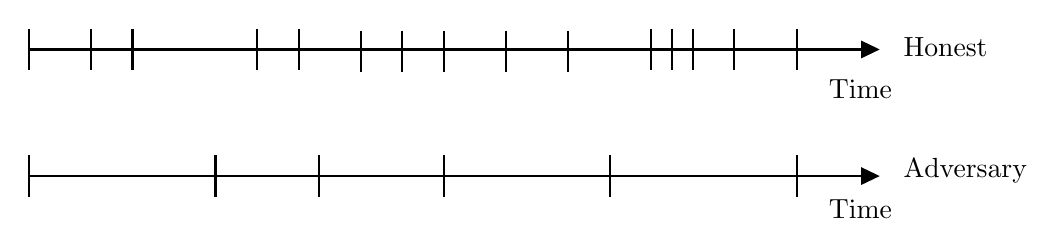
\begin{tikzpicture}[x=0.75pt,y=0.75pt,yscale=-1,xscale=1]
%uncomment if require: \path (0,112); %set diagram left start at 0, and has height of 112

%Straight Lines [id:da23525023892191266]
\draw    (140,20) -- (547,20) ;
\draw [shift={(550,20)}, rotate = 180] [fill={rgb, 255:red, 0; green, 0; blue, 0 }  ][line width=0.08]  [draw opacity=0] (8.93,-4.29) -- (0,0) -- (8.93,4.29) -- cycle    ;
%Straight Lines [id:da7960445132740581]
\draw    (140,10) -- (140,30) ;
%Straight Lines [id:da29783337527097675]
\draw    (270,10) -- (270,30) ;
%Straight Lines [id:da33677894078119586]
\draw    (190,10) -- (190,30) ;
%Straight Lines [id:da5399367214918731]
\draw    (370,11) -- (370,31) ;
%Straight Lines [id:da09675758542474289]
\draw    (440,10) -- (440,30) ;
%Straight Lines [id:da5769918595193868]
\draw    (450,10) -- (450,30) ;
%Straight Lines [id:da31319754434895075]
\draw    (460,10) -- (460,30) ;
%Straight Lines [id:da33141985537928864]
\draw    (510,10) -- (510,30) ;
%Straight Lines [id:da11800923635182015]
\draw    (140,81) -- (547,81) ;
\draw [shift={(550,81)}, rotate = 180] [fill={rgb, 255:red, 0; green, 0; blue, 0 }  ][line width=0.08]  [draw opacity=0] (8.93,-4.29) -- (0,0) -- (8.93,4.29) -- cycle    ;
%Straight Lines [id:da07789537672362723]
\draw    (140,71) -- (140,91) ;
%Straight Lines [id:da8372706005219659]
\draw    (280,71) -- (280,91) ;
%Straight Lines [id:da29756814685721467]
\draw    (230,71) -- (230,91) ;
%Straight Lines [id:da86063133847938]
\draw    (340,71) -- (340,91) ;
%Straight Lines [id:da599322584965772]
\draw    (420,71) -- (420,91) ;
%Straight Lines [id:da03302559846585229]
\draw    (510,71) -- (510,91) ;
%Straight Lines [id:da21596375747665641]
\draw    (340,11) -- (340,31) ;
%Straight Lines [id:da8449429552182337]
\draw    (320,11) -- (320,31) ;
%Straight Lines [id:da022987682318881708]
\draw    (250,10) -- (250,30) ;
%Straight Lines [id:da9209115770539547]
\draw    (170,10) -- (170,30) ;
%Straight Lines [id:da03134967763740537]
\draw    (300,11) -- (300,31) ;
%Straight Lines [id:da8935379151898348]
\draw    (400,11) -- (400,31) ;
%Straight Lines [id:da957853887353433]
\draw    (480,10) -- (480,30) ;

% Text Node
\draw (524,33) node [anchor=north west][inner sep=0.75pt]   [align=left] {Time};
% Text Node
\draw (560,13) node [anchor=north west][inner sep=0.75pt]   [align=left] {Honest};
% Text Node
\draw (524,91) node [anchor=north west][inner sep=0.75pt]   [align=left] {Time};
% Text Node
\draw (560,71) node [anchor=north west][inner sep=0.75pt]   [align=left] {Adversary};


\end{tikzpicture}
    \caption{Block production of honest nodes vs. the adversary}
    \label{fig:Honest block production power}
\end{figure}

\begin{figure}[H]
	\centering
\tikzset{every picture/.style={line width=0.75pt}} %set default line width to 0.75pt

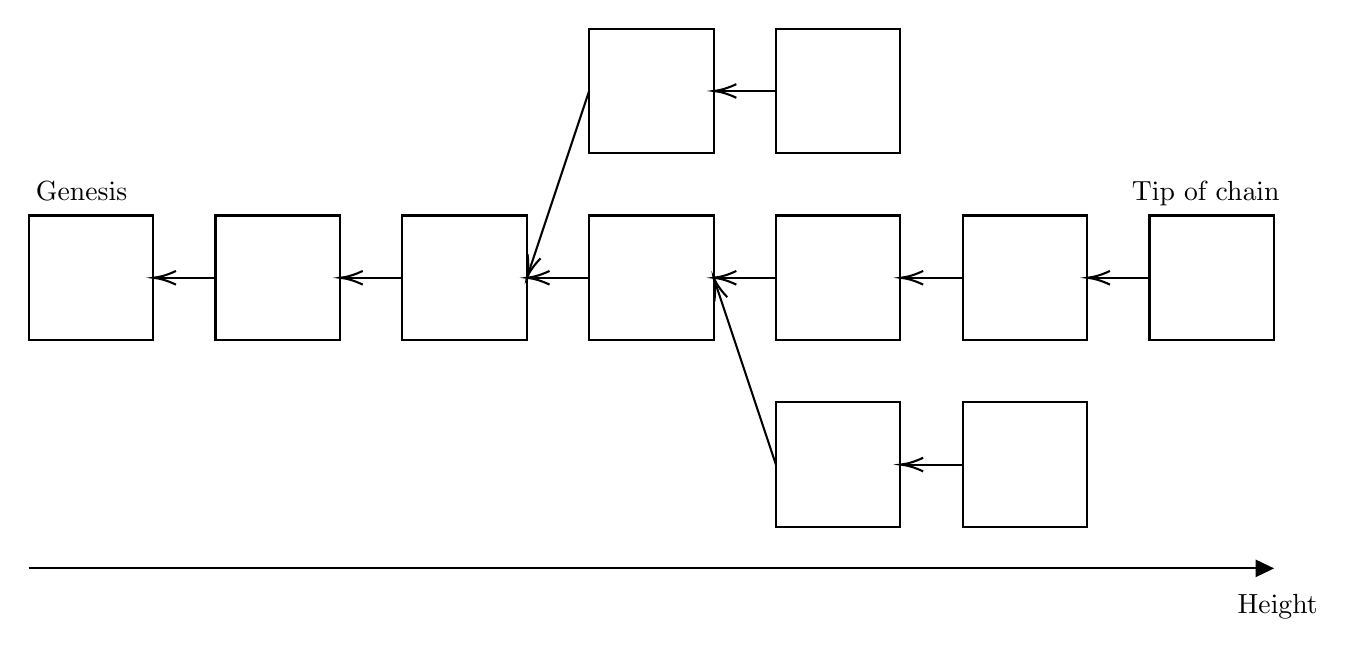
\begin{tikzpicture}[x=0.75pt,y=0.75pt,yscale=-1,xscale=1]
%uncomment if require: \path (0,317); %set diagram left start at 0, and has height of 317

%Shape: Square [id:dp5553489928334188]
\draw   (20,100) -- (80,100) -- (80,160) -- (20,160) -- cycle ;
%Straight Lines [id:da02867875054034763]
\draw    (110,130) -- (82,130) ;
\draw [shift={(80,130)}, rotate = 360] [color={rgb, 255:red, 0; green, 0; blue, 0 }  ][line width=0.75]    (10.93,-3.29) .. controls (6.95,-1.4) and (3.31,-0.3) .. (0,0) .. controls (3.31,0.3) and (6.95,1.4) .. (10.93,3.29)   ;
%Shape: Square [id:dp49650358706771236]
\draw   (110,100) -- (170,100) -- (170,160) -- (110,160) -- cycle ;
%Straight Lines [id:da05327516325435977]
\draw    (200,130) -- (172,130) ;
\draw [shift={(170,130)}, rotate = 360] [color={rgb, 255:red, 0; green, 0; blue, 0 }  ][line width=0.75]    (10.93,-3.29) .. controls (6.95,-1.4) and (3.31,-0.3) .. (0,0) .. controls (3.31,0.3) and (6.95,1.4) .. (10.93,3.29)   ;
%Shape: Square [id:dp44489240803143804]
\draw   (200,100) -- (260,100) -- (260,160) -- (200,160) -- cycle ;
%Straight Lines [id:da7431038331619342]
\draw    (290,130) -- (262,130) ;
\draw [shift={(260,130)}, rotate = 360] [color={rgb, 255:red, 0; green, 0; blue, 0 }  ][line width=0.75]    (10.93,-3.29) .. controls (6.95,-1.4) and (3.31,-0.3) .. (0,0) .. controls (3.31,0.3) and (6.95,1.4) .. (10.93,3.29)   ;
%Shape: Square [id:dp540021094447644]
\draw   (290,100) -- (350,100) -- (350,160) -- (290,160) -- cycle ;
%Shape: Square [id:dp86801051079086]
\draw   (380,190) -- (440,190) -- (440,250) -- (380,250) -- cycle ;
%Straight Lines [id:da6968247771293123]
\draw    (380,220) -- (350.63,131.9) ;
\draw [shift={(350,130)}, rotate = 71.57] [color={rgb, 255:red, 0; green, 0; blue, 0 }  ][line width=0.75]    (10.93,-3.29) .. controls (6.95,-1.4) and (3.31,-0.3) .. (0,0) .. controls (3.31,0.3) and (6.95,1.4) .. (10.93,3.29)   ;
%Straight Lines [id:da10617452462704291]
\draw    (470,220) -- (442,220) ;
\draw [shift={(440,220)}, rotate = 360] [color={rgb, 255:red, 0; green, 0; blue, 0 }  ][line width=0.75]    (10.93,-3.29) .. controls (6.95,-1.4) and (3.31,-0.3) .. (0,0) .. controls (3.31,0.3) and (6.95,1.4) .. (10.93,3.29)   ;
%Shape: Square [id:dp013136466066319574]
\draw   (470,190) -- (530,190) -- (530,250) -- (470,250) -- cycle ;
%Straight Lines [id:da5171350092317244]
\draw    (380,130) -- (352,130) ;
\draw [shift={(350,130)}, rotate = 360] [color={rgb, 255:red, 0; green, 0; blue, 0 }  ][line width=0.75]    (10.93,-3.29) .. controls (6.95,-1.4) and (3.31,-0.3) .. (0,0) .. controls (3.31,0.3) and (6.95,1.4) .. (10.93,3.29)   ;
%Shape: Square [id:dp6846062105068249]
\draw   (380,100) -- (440,100) -- (440,160) -- (380,160) -- cycle ;
%Shape: Square [id:dp863890663182566]
\draw   (290,10) -- (350,10) -- (350,70) -- (290,70) -- cycle ;
%Straight Lines [id:da04868739915580034]
\draw    (290,40) -- (260.63,128.1) ;
\draw [shift={(260,130)}, rotate = 288.43] [color={rgb, 255:red, 0; green, 0; blue, 0 }  ][line width=0.75]    (10.93,-3.29) .. controls (6.95,-1.4) and (3.31,-0.3) .. (0,0) .. controls (3.31,0.3) and (6.95,1.4) .. (10.93,3.29)   ;
%Straight Lines [id:da36373788691107434]
\draw    (380,40) -- (352,40) ;
\draw [shift={(350,40)}, rotate = 360] [color={rgb, 255:red, 0; green, 0; blue, 0 }  ][line width=0.75]    (10.93,-3.29) .. controls (6.95,-1.4) and (3.31,-0.3) .. (0,0) .. controls (3.31,0.3) and (6.95,1.4) .. (10.93,3.29)   ;
%Shape: Square [id:dp8457049773626129]
\draw   (380,10) -- (440,10) -- (440,70) -- (380,70) -- cycle ;
%Shape: Square [id:dp746865970815856]
\draw   (470,100) -- (530,100) -- (530,160) -- (470,160) -- cycle ;
%Straight Lines [id:da7437715956006345]
\draw    (560,130) -- (532,130) ;
\draw [shift={(530,130)}, rotate = 360] [color={rgb, 255:red, 0; green, 0; blue, 0 }  ][line width=0.75]    (10.93,-3.29) .. controls (6.95,-1.4) and (3.31,-0.3) .. (0,0) .. controls (3.31,0.3) and (6.95,1.4) .. (10.93,3.29)   ;
%Shape: Square [id:dp9434239793653232]
\draw   (560,100) -- (620,100) -- (620,160) -- (560,160) -- cycle ;
%Straight Lines [id:da06385468421590201]
\draw    (470,130) -- (442,130) ;
\draw [shift={(440,130)}, rotate = 360] [color={rgb, 255:red, 0; green, 0; blue, 0 }  ][line width=0.75]    (10.93,-3.29) .. controls (6.95,-1.4) and (3.31,-0.3) .. (0,0) .. controls (3.31,0.3) and (6.95,1.4) .. (10.93,3.29)   ;
%Straight Lines [id:da4081512417331501]
\draw    (20,270) -- (617,270) ;
\draw [shift={(620,270)}, rotate = 180] [fill={rgb, 255:red, 0; green, 0; blue, 0 }  ][line width=0.08]  [draw opacity=0] (8.93,-4.29) -- (0,0) -- (8.93,4.29) -- cycle    ;
%Straight Lines [id:da6329335012714348]
% \draw    (20,260) -- (20,280) ;
%Straight Lines [id:da5452663697779279]
% \draw    (110,260) -- (110,280) ;
%Straight Lines [id:da8605249971113638]
% \draw    (200,260) -- (200,280) ;
%Straight Lines [id:da8480595218681781]
% \draw    (290,260) -- (290,280) ;
%Straight Lines [id:da13016480179291512]
% \draw    (380,260) -- (380,280) ;
%Straight Lines [id:da0032258538987217644]
% \draw    (470,260) -- (470,280) ;
%Straight Lines [id:da08791748462517157]
% \draw    (560,260) -- (560,280) ;

% Text Node
\draw (550,82) node [anchor=north west][inner sep=0.75pt]   [align=left] {Tip of chain};
% Text Node
\draw (601,281) node [anchor=north west][inner sep=0.75pt]   [align=left] {Height};
% Text Node
\draw (22,82) node [anchor=north west][inner sep=0.75pt]   [align=left] {Genesis};
% Text Node
% \draw (15,282.4) node [anchor=north west][inner sep=0.75pt]    {$0$};
% % Text Node
% \draw (105,282.4) node [anchor=north west][inner sep=0.75pt]    {$1$};
% % Text Node
% \draw (195,282.4) node [anchor=north west][inner sep=0.75pt]    {$2$};
% % Text Node
% \draw (285,283.4) node [anchor=north west][inner sep=0.75pt]    {$3$};
% % Text Node
% \draw (375,282.4) node [anchor=north west][inner sep=0.75pt]    {$4$};
% % Text Node
% \draw (465,282.4) node [anchor=north west][inner sep=0.75pt]    {$5$};
% % Text Node
% \draw (555,282.4) node [anchor=north west][inner sep=0.75pt]    {$6$};


\end{tikzpicture}
	\caption{Block trees and the longest chain rule. There may be temporary forks because of conflicting blocks. But, the occurrence of convergence opportunities ensures that eventually, there will be a unique tip of the longest chain.}
	\label{fig:Block tree}  %Tag for referring to figure in text.
\end{figure}

\section{Coinbase Transactions}

While we have successfully implemented a way to validate ownership of money in a decentralized manner, we have yet to see how to tackle the creation of money.

To do so, we introduce the notion of a ``coinbase transaction''. This transaction is uniquely present in every block. The miner creates this transaction, and can reward any public key they want with an amount less than or equal to a fixed amount $f$ (the block reward) determined by the network plus transaction fees (the fee reward). These fees correspond to the difference between inputs and outputs in each transaction confirmed in the block. Due to the weak law of conservation, recall that there can be a difference between the sum of the inputs and the sum of the outputs in each transaction. This difference is paid out as fees. In other words, the miner can create a transaction with no input and one output with an amount $a$ respecting the following equation:
\begin{equation}
    a \leq f + \sum_{i \in {\text{input}}} i.v - \sum_{o \in {\text{ouput}}} o.v
\end{equation}
where the sum is over all transactions in the block.
In our Marabu protocol, we use $f = 50$ bu.

Finally, to avoid multiple identical transactions that would have the same hash as a result of having the same amount and same public key output, an additional \emph{height} parameter is included in the coinbase transaction. This parameter corresponds to the number of blocks that this block is away from genesis.

\section{Verifying Objects}

\subsection{Verifying a Block}

Upon receiving a block, a honest node should:
\begin{enumerate}
    \item Verify the proof of work (and do this first to avoid spam attacks).
    \item Verify the parent block recursively (and if it does not exist locally, request it from the network).
    \item Verify the transactions inside the block, including the coinbase transaction (and if it does not have them, request them from the network).
\end{enumerate}

\subsection{Verifying a Chain}

Upon receiving a chain, a honest node should:
\begin{enumerate}
    \item Verify each block in the chain.
    \item Check that it starts with genesis (or is connected to a block known to be connected to genesis).
    \item Adopt the longest chain or one of the longest chains.
\end{enumerate}

\subsection{Verifying a Regular Transaction}

See lecture 4

\subsection{Verifying a Coinbase Transaction}

A valid coinbase transaction must:
\begin{enumerate}
    \item be the only one in that block,
    \item be the first transaction in the block,
    \item have no input and exactly one output,
    \item have a value which is less than or equal to the sum of the fixed block reward and the difference between the input and output amounts of all other transactions in the block,
    \item not be spent in the same block.
\end{enumerate}

\section{Comparing Transactions and Blocks}

Now that we understand how blocks and transactions work, it is worth drawing parallels between the two.
\begin{center}
\begin{tabular}{ |c|c|c| }
  \hline
  & \textbf{Transaction} & \textbf{Block} \\
  \hline
  \textbf{Inductive base} & Coinbase & Genesis \\
  \hline
  \textbf{Inductive hypothesis} & Outpoint UTXO & Previous ID ($s$) \\
  \hline
  \textbf{Inductive step} & \makecell{Consuming produced UTXO \\ Signatures \\ Conservation laws} & \makecell{Proof of Work \\ Causality \\ Transactions} \\
  \hline
\end{tabular}
\end{center}

\section{Updating the UTXO}

For each received transaction, if the transaction is valid, apply the transaction to the previous UTXO to get the new UTXO.

For each reveived block, apply each transaction of the block to the previous UTXO. If at any point a transaction is invalid, reject the entire block and revert to the previous UTXO.

For all transactions not yet in a block, add them to a mempool with a temporary UTXO which starts as the same UTXO as the current longest chain tip. These transactions are added in the order in which they are received. If the transaction is invalid with respect to the current UTXO, reject it. When mining a block, use all of the transactions in the mempool to create this block.

Upon receiving a block at the tip of the current longest chain, validate the block and update the UTXO. Also update the mempool and temporary UTXO by applying transactions in the block or removing any transaction that is now either invalid or already in the newly received block.

Upon receiving a block which changes the longest chain to another chain, set the UTXO to the fork between the current longest chain and this new chain (by undoing all transactions after the fork in the current chain). Then, go through each block until the tip in the new longest chain and update the UTXO. If at any point, a block is invalid, reject the new chain and revert to the previous chain and previous UTXO. If all blocks after the fork in the new longest chain are valid, update the mempool by starting with the UTXO at the tip of the new longest chain, applying every valid transaction in the previous longest chain that is not present in the new longest chain, then applying all the still-valid transactions that were previously in the mempool. This process of adopting the longest chain is shown in Figure~\ref{fig:UTXOChainChange}. \\

\begin{figure}[H]
    \centering
\tikzset{every picture/.style={line width=0.75pt}} %set default line width to 0.75pt

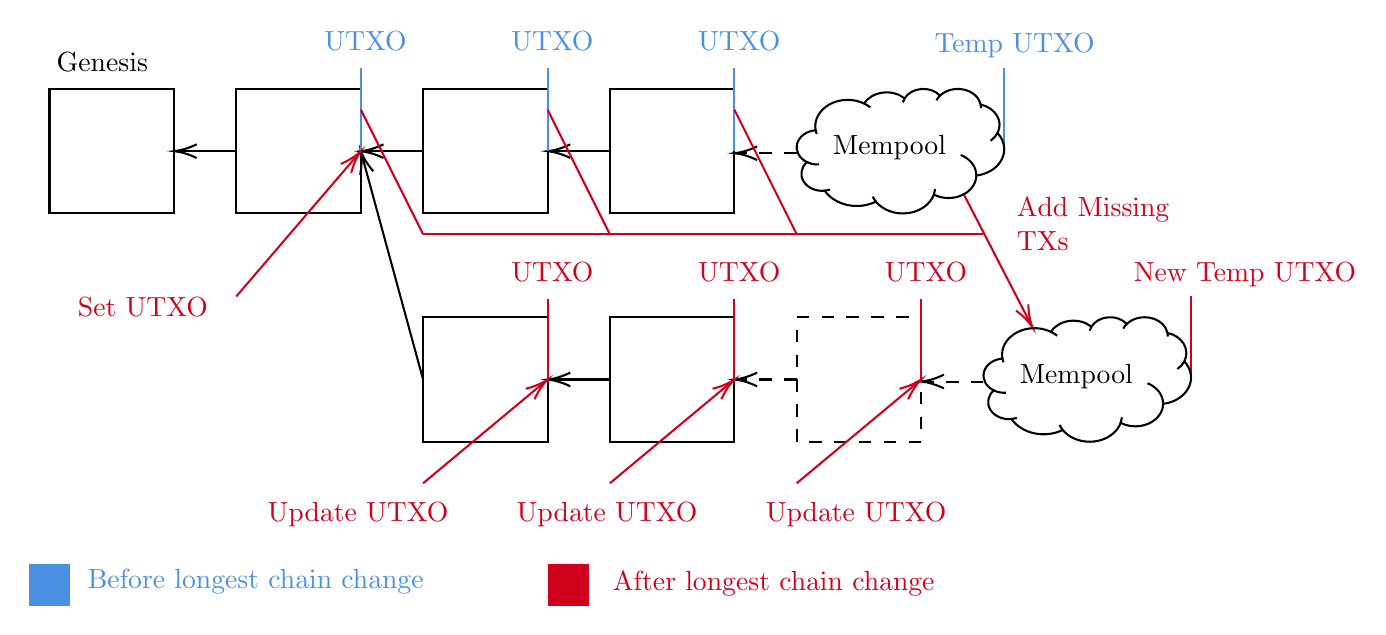
\begin{tikzpicture}[x=0.75pt,y=0.75pt,yscale=-1,xscale=1]
%uncomment if require: \path (0,303); %set diagram left start at 0, and has height of 303

%Shape: Square [id:dp6521466830611065]
\draw   (20,41) -- (80,41) -- (80,101) -- (20,101) -- cycle ;
%Straight Lines [id:da7819102316771764]
\draw    (110,71) -- (82,71) ;
\draw [shift={(80,71)}, rotate = 360] [color={rgb, 255:red, 0; green, 0; blue, 0 }  ][line width=0.75]    (10.93,-3.29) .. controls (6.95,-1.4) and (3.31,-0.3) .. (0,0) .. controls (3.31,0.3) and (6.95,1.4) .. (10.93,3.29)   ;
%Shape: Square [id:dp6182477130409076]
\draw   (110,41) -- (170,41) -- (170,101) -- (110,101) -- cycle ;
%Straight Lines [id:da22654224529120404]
\draw    (200,71) -- (172,71) ;
\draw [shift={(170,71)}, rotate = 360] [color={rgb, 255:red, 0; green, 0; blue, 0 }  ][line width=0.75]    (10.93,-3.29) .. controls (6.95,-1.4) and (3.31,-0.3) .. (0,0) .. controls (3.31,0.3) and (6.95,1.4) .. (10.93,3.29)   ;
%Shape: Square [id:dp02337826181900904]
\draw   (200,41) -- (260,41) -- (260,101) -- (200,101) -- cycle ;
%Straight Lines [id:da15734675441574208]
\draw    (290,71) -- (262,71) ;
\draw [shift={(260,71)}, rotate = 360] [color={rgb, 255:red, 0; green, 0; blue, 0 }  ][line width=0.75]    (10.93,-3.29) .. controls (6.95,-1.4) and (3.31,-0.3) .. (0,0) .. controls (3.31,0.3) and (6.95,1.4) .. (10.93,3.29)   ;
%Shape: Square [id:dp840092006051874]
\draw   (290,41) -- (350,41) -- (350,101) -- (290,101) -- cycle ;
%Shape: Square [id:dp801014946422226]
\draw   (200,151) -- (260,151) -- (260,211) -- (200,211) -- cycle ;
%Straight Lines [id:da9537380349189299]
\draw    (200,181) -- (170.53,72.93) ;
\draw [shift={(170,71)}, rotate = 74.74] [color={rgb, 255:red, 0; green, 0; blue, 0 }  ][line width=0.75]    (10.93,-3.29) .. controls (6.95,-1.4) and (3.31,-0.3) .. (0,0) .. controls (3.31,0.3) and (6.95,1.4) .. (10.93,3.29)   ;
%Straight Lines [id:da8212782642294261]
\draw    (290,181) -- (262,181) ;
\draw [shift={(260,181)}, rotate = 360] [color={rgb, 255:red, 0; green, 0; blue, 0 }  ][line width=0.75]    (10.93,-3.29) .. controls (6.95,-1.4) and (3.31,-0.3) .. (0,0) .. controls (3.31,0.3) and (6.95,1.4) .. (10.93,3.29)   ;
%Shape: Square [id:dp22084257855473166]
\draw   (290,151) -- (350,151) -- (350,211) -- (290,211) -- cycle ;
%Straight Lines [id:da9533389147995392]
\draw  [dash pattern={on 4.5pt off 4.5pt}]  (380,181) -- (352,181) ;
\draw [shift={(350,181)}, rotate = 360] [color={rgb, 255:red, 0; green, 0; blue, 0 }  ][line width=0.75]    (10.93,-3.29) .. controls (6.95,-1.4) and (3.31,-0.3) .. (0,0) .. controls (3.31,0.3) and (6.95,1.4) .. (10.93,3.29)   ;
%Shape: Square [id:dp9382911344304163]
\draw  [dash pattern={on 4.5pt off 4.5pt}] (380,151) -- (440,151) -- (440,211) -- (380,211) -- cycle ;
%Straight Lines [id:da7513116931470782]
\draw [color={rgb, 255:red, 74; green, 144; blue, 226 }  ,draw opacity=1 ]   (170,31) -- (170,71) ;
%Straight Lines [id:da7430295277757613]
\draw [color={rgb, 255:red, 74; green, 144; blue, 226 }  ,draw opacity=1 ]   (260,31) -- (260,71) ;
%Straight Lines [id:da11052295583016747]
\draw [color={rgb, 255:red, 74; green, 144; blue, 226 }  ,draw opacity=1 ]   (350,31) -- (350,71) ;
%Straight Lines [id:da8715298181677615]
\draw [color={rgb, 255:red, 208; green, 2; blue, 27 }  ,draw opacity=1 ]   (260,142) -- (260,182) ;
%Straight Lines [id:da9627172266750117]
\draw [color={rgb, 255:red, 208; green, 2; blue, 27 }  ,draw opacity=1 ]   (350,142) -- (350,182) ;
%Straight Lines [id:da3023883615554328]
\draw [color={rgb, 255:red, 208; green, 2; blue, 27 }  ,draw opacity=1 ]   (110,141) -- (168.7,72.52) ;
\draw [shift={(170,71)}, rotate = 130.6] [color={rgb, 255:red, 208; green, 2; blue, 27 }  ,draw opacity=1 ][line width=0.75]    (10.93,-3.29) .. controls (6.95,-1.4) and (3.31,-0.3) .. (0,0) .. controls (3.31,0.3) and (6.95,1.4) .. (10.93,3.29)   ;
%Straight Lines [id:da9901888064889268]
\draw [color={rgb, 255:red, 208; green, 2; blue, 27 }  ,draw opacity=1 ]   (200,231) -- (214.92,218.57) -- (258.46,182.28) ;
\draw [shift={(260,181)}, rotate = 140.19] [color={rgb, 255:red, 208; green, 2; blue, 27 }  ,draw opacity=1 ][line width=0.75]    (10.93,-3.29) .. controls (6.95,-1.4) and (3.31,-0.3) .. (0,0) .. controls (3.31,0.3) and (6.95,1.4) .. (10.93,3.29)   ;
%Straight Lines [id:da7470962668798595]
\draw [color={rgb, 255:red, 208; green, 2; blue, 27 }  ,draw opacity=1 ]   (440,142) -- (440,182) ;
%Straight Lines [id:da5600163205713113]
\draw [color={rgb, 255:red, 208; green, 2; blue, 27 }  ,draw opacity=1 ]   (460.25,91.25) -- (492.75,154.22) ;
\draw [shift={(493.67,156)}, rotate = 242.7] [color={rgb, 255:red, 208; green, 2; blue, 27 }  ,draw opacity=1 ][line width=0.75]    (10.93,-3.29) .. controls (6.95,-1.4) and (3.31,-0.3) .. (0,0) .. controls (3.31,0.3) and (6.95,1.4) .. (10.93,3.29)   ;
%Straight Lines [id:da535323812611922]
\draw  [dash pattern={on 4.5pt off 4.5pt}]  (380,71.99) -- (352,71.99) ;
\draw [shift={(350,71.99)}, rotate = 360] [color={rgb, 255:red, 0; green, 0; blue, 0 }  ][line width=0.75]    (10.93,-3.29) .. controls (6.95,-1.4) and (3.31,-0.3) .. (0,0) .. controls (3.31,0.3) and (6.95,1.4) .. (10.93,3.29)   ;
%Straight Lines [id:da10474572702800766]
\draw  [dash pattern={on 4.5pt off 4.5pt}]  (470,181.99) -- (442,181.99) ;
\draw [shift={(440,181.99)}, rotate = 360] [color={rgb, 255:red, 0; green, 0; blue, 0 }  ][line width=0.75]    (10.93,-3.29) .. controls (6.95,-1.4) and (3.31,-0.3) .. (0,0) .. controls (3.31,0.3) and (6.95,1.4) .. (10.93,3.29)   ;
%Straight Lines [id:da98694418087908]
\draw [color={rgb, 255:red, 208; green, 2; blue, 27 }  ,draw opacity=1 ]   (170,51) -- (200,111) ;
%Straight Lines [id:da7736807885577637]
\draw [color={rgb, 255:red, 208; green, 2; blue, 27 }  ,draw opacity=1 ]   (260,51) -- (290,111) ;
%Straight Lines [id:da5079296287543524]
\draw [color={rgb, 255:red, 208; green, 2; blue, 27 }  ,draw opacity=1 ]   (350,51) -- (380,111) ;
%Straight Lines [id:da970296926623833]
\draw [color={rgb, 255:red, 208; green, 2; blue, 27 }  ,draw opacity=1 ]   (200,111) -- (470,111) ;
%Straight Lines [id:da16682911027696634]
\draw [color={rgb, 255:red, 74; green, 144; blue, 226 }  ,draw opacity=1 ]   (480,31) -- (480,71) ;
%Straight Lines [id:da9543785277219905]
\draw [color={rgb, 255:red, 208; green, 2; blue, 27 }  ,draw opacity=1 ]   (570,141) -- (570,181) ;
%Shape: Cloud [id:dp30012303953626596]
\draw   (389.1,60.75) .. controls (388.29,55.92) and (390.94,51.13) .. (395.91,48.42) .. controls (400.88,45.71) and (407.31,45.56) .. (412.46,48.03) .. controls (414.29,45.21) and (417.63,43.27) .. (421.48,42.79) .. controls (425.32,42.3) and (429.22,43.33) .. (432,45.57) .. controls (433.55,43.02) and (436.61,41.31) .. (440.08,41.04) .. controls (443.55,40.77) and (446.94,41.98) .. (449.05,44.25) .. controls (451.86,41.55) and (456.33,40.41) .. (460.53,41.33) .. controls (464.73,42.25) and (467.9,45.06) .. (468.67,48.55) .. controls (472.11,49.31) and (474.98,51.27) .. (476.53,53.9) .. controls (478.08,56.53) and (478.16,59.58) .. (476.76,62.27) .. controls (480.15,65.88) and (480.94,70.68) .. (478.84,74.89) .. controls (476.74,79.11) and (472.06,82.09) .. (466.55,82.74) .. controls (466.51,86.69) and (463.86,90.32) .. (459.62,92.22) .. controls (455.38,94.12) and (450.21,94.01) .. (446.1,91.91) .. controls (444.35,96.65) and (439.43,100.13) .. (433.46,100.86) .. controls (427.48,101.59) and (421.54,99.43) .. (418.18,95.32) .. controls (414.07,97.34) and (409.14,97.93) .. (404.49,96.94) .. controls (399.85,95.95) and (395.89,93.46) .. (393.5,90.05) .. controls (389.3,90.45) and (385.24,88.67) .. (383.33,85.59) .. controls (381.42,82.51) and (382.08,78.79) .. (384.97,76.27) .. controls (381.22,74.47) and (379.31,70.89) .. (380.23,67.4) .. controls (381.15,63.92) and (384.69,61.31) .. (389.02,60.94) ; \draw   (384.97,76.27) .. controls (386.74,77.13) and (388.78,77.51) .. (390.83,77.38)(393.5,90.05) .. controls (394.38,89.96) and (395.24,89.79) .. (396.07,89.52)(418.18,95.32) .. controls (417.56,94.56) and (417.05,93.75) .. (416.64,92.9)(446.1,91.91) .. controls (446.42,91.05) and (446.62,90.16) .. (446.72,89.26)(466.55,82.74) .. controls (466.59,78.53) and (463.67,74.67) .. (459.04,72.83)(476.76,62.27) .. controls (476.01,63.7) and (474.86,64.97) .. (473.41,65.98)(468.67,48.55) .. controls (468.79,49.12) and (468.85,49.71) .. (468.84,50.3)(449.05,44.25) .. controls (448.35,44.92) and (447.77,45.68) .. (447.34,46.49)(432,45.57) .. controls (431.62,46.18) and (431.34,46.83) .. (431.17,47.5)(412.46,48.03) .. controls (413.55,48.55) and (414.56,49.18) .. (415.46,49.9)(389.1,60.75) .. controls (389.21,61.42) and (389.39,62.08) .. (389.62,62.72) ;
%Shape: Cloud [id:dp9947625990800526]
\draw   (479.1,170.75) .. controls (478.29,165.92) and (480.94,161.13) .. (485.91,158.42) .. controls (490.88,155.71) and (497.31,155.56) .. (502.46,158.03) .. controls (504.29,155.21) and (507.63,153.27) .. (511.48,152.79) .. controls (515.32,152.3) and (519.22,153.33) .. (522,155.57) .. controls (523.55,153.02) and (526.61,151.31) .. (530.08,151.04) .. controls (533.55,150.77) and (536.94,151.98) .. (539.05,154.25) .. controls (541.86,151.55) and (546.33,150.41) .. (550.53,151.33) .. controls (554.73,152.25) and (557.9,155.06) .. (558.67,158.55) .. controls (562.11,159.31) and (564.98,161.27) .. (566.53,163.9) .. controls (568.08,166.53) and (568.16,169.58) .. (566.76,172.27) .. controls (570.15,175.88) and (570.94,180.68) .. (568.84,184.89) .. controls (566.74,189.11) and (562.06,192.09) .. (556.55,192.74) .. controls (556.51,196.69) and (553.86,200.32) .. (549.62,202.22) .. controls (545.38,204.12) and (540.21,204.01) .. (536.1,201.91) .. controls (534.35,206.65) and (529.43,210.13) .. (523.46,210.86) .. controls (517.48,211.59) and (511.54,209.43) .. (508.18,205.32) .. controls (504.07,207.34) and (499.14,207.93) .. (494.49,206.94) .. controls (489.85,205.95) and (485.89,203.46) .. (483.5,200.05) .. controls (479.3,200.45) and (475.24,198.67) .. (473.33,195.59) .. controls (471.42,192.51) and (472.08,188.79) .. (474.97,186.27) .. controls (471.22,184.47) and (469.31,180.89) .. (470.23,177.4) .. controls (471.15,173.92) and (474.69,171.31) .. (479.02,170.94) ; \draw   (474.97,186.27) .. controls (476.74,187.13) and (478.78,187.51) .. (480.83,187.38)(483.5,200.05) .. controls (484.38,199.96) and (485.24,199.79) .. (486.07,199.52)(508.18,205.32) .. controls (507.56,204.56) and (507.05,203.75) .. (506.64,202.9)(536.1,201.91) .. controls (536.42,201.05) and (536.62,200.16) .. (536.72,199.26)(556.55,192.74) .. controls (556.59,188.53) and (553.67,184.67) .. (549.04,182.83)(566.76,172.27) .. controls (566.01,173.7) and (564.86,174.97) .. (563.41,175.98)(558.67,158.55) .. controls (558.79,159.12) and (558.85,159.71) .. (558.84,160.3)(539.05,154.25) .. controls (538.35,154.92) and (537.77,155.68) .. (537.34,156.49)(522,155.57) .. controls (521.62,156.18) and (521.34,156.83) .. (521.17,157.5)(502.46,158.03) .. controls (503.55,158.55) and (504.56,159.18) .. (505.46,159.9)(479.1,170.75) .. controls (479.21,171.42) and (479.39,172.08) .. (479.62,172.72) ;
%Straight Lines [id:da21490206379605126]
\draw [color={rgb, 255:red, 208; green, 2; blue, 27 }  ,draw opacity=1 ]   (290,231) -- (304.92,218.57) -- (348.46,182.28) ;
\draw [shift={(350,181)}, rotate = 140.19] [color={rgb, 255:red, 208; green, 2; blue, 27 }  ,draw opacity=1 ][line width=0.75]    (10.93,-3.29) .. controls (6.95,-1.4) and (3.31,-0.3) .. (0,0) .. controls (3.31,0.3) and (6.95,1.4) .. (10.93,3.29)   ;
%Straight Lines [id:da21349308780257403]
\draw [color={rgb, 255:red, 208; green, 2; blue, 27 }  ,draw opacity=1 ]   (380,231) -- (394.92,218.57) -- (438.46,182.28) ;
\draw [shift={(440,181)}, rotate = 140.19] [color={rgb, 255:red, 208; green, 2; blue, 27 }  ,draw opacity=1 ][line width=0.75]    (10.93,-3.29) .. controls (6.95,-1.4) and (3.31,-0.3) .. (0,0) .. controls (3.31,0.3) and (6.95,1.4) .. (10.93,3.29)   ;
%Shape: Rectangle [id:dp7810240526075007]
\draw  [draw opacity=0][fill={rgb, 255:red, 208; green, 2; blue, 27 }  ,fill opacity=1 ] (260,270) -- (280,270) -- (280,290) -- (260,290) -- cycle ;
%Shape: Rectangle [id:dp19832461992006012]
\draw  [draw opacity=0][fill={rgb, 255:red, 74; green, 144; blue, 226 }  ,fill opacity=1 ] (10,270) -- (30,270) -- (30,290) -- (10,290) -- cycle ;

% Text Node
\draw (151,12) node [anchor=north west][inner sep=0.75pt]   [align=left] {\textcolor[rgb]{0.29,0.56,0.89}{UTXO}};
% Text Node
\draw (241,12) node [anchor=north west][inner sep=0.75pt]   [align=left] {\textcolor[rgb]{0.29,0.56,0.89}{UTXO}};
% Text Node
\draw (331,12) node [anchor=north west][inner sep=0.75pt]   [align=left] {\textcolor[rgb]{0.29,0.56,0.89}{UTXO}};
% Text Node
\draw (396,62) node [anchor=north west][inner sep=0.75pt]   [align=left] {Mempool};
% Text Node
\draw (241,123) node [anchor=north west][inner sep=0.75pt]  [color={rgb, 255:red, 208; green, 2; blue, 27 }  ,opacity=1 ] [align=left] {\textcolor[rgb]{0.82,0.01,0.11}{UTXO}};
% Text Node
\draw (331,123) node [anchor=north west][inner sep=0.75pt]  [color={rgb, 255:red, 208; green, 2; blue, 27 }  ,opacity=1 ] [align=left] {\textcolor[rgb]{0.82,0.01,0.11}{UTXO}};
% Text Node
\draw (70,146) node  [color={rgb, 255:red, 208; green, 2; blue, 27 }  ,opacity=1 ] [align=left] {\begin{minipage}[lt]{54.4pt}\setlength\topsep{0pt}
Set UTXO
\end{minipage}};
% Text Node
\draw (175,246) node  [color={rgb, 255:red, 208; green, 2; blue, 27 }  ,opacity=1 ] [align=left] {\begin{minipage}[lt]{74.8pt}\setlength\topsep{0pt}
Update UTXO
\end{minipage}};
% Text Node
\draw (421,123) node [anchor=north west][inner sep=0.75pt]  [color={rgb, 255:red, 208; green, 2; blue, 27 }  ,opacity=1 ] [align=left] {\textcolor[rgb]{0.82,0.01,0.11}{UTXO}};
% Text Node
\draw (445,13) node [anchor=north west][inner sep=0.75pt]   [align=left] {\textcolor[rgb]{0.29,0.56,0.89}{Temp UTXO}};
% Text Node
\draw (545,106) node  [color={rgb, 255:red, 208; green, 2; blue, 27 }  ,opacity=1 ] [align=left] {\begin{minipage}[lt]{88.4pt}\setlength\topsep{0pt}
Add Missing\\TXs
\end{minipage}};
% Text Node
\draw (541,123) node [anchor=north west][inner sep=0.75pt]  [color={rgb, 255:red, 208; green, 2; blue, 27 }  ,opacity=1 ] [align=left] {\textcolor[rgb]{0.82,0.01,0.11}{New Temp UTXO}};
% Text Node
\draw (486,172) node [anchor=north west][inner sep=0.75pt]   [align=left] {Mempool};
% Text Node
\draw (290,272) node [anchor=north west][inner sep=0.75pt]  [color={rgb, 255:red, 208; green, 2; blue, 27 }  ,opacity=1 ] [align=left] {After longest chain change};
% Text Node
\draw (295,246) node  [color={rgb, 255:red, 208; green, 2; blue, 27 }  ,opacity=1 ] [align=left] {\begin{minipage}[lt]{74.8pt}\setlength\topsep{0pt}
Update UTXO
\end{minipage}};
% Text Node
\draw (415,246) node  [color={rgb, 255:red, 208; green, 2; blue, 27 }  ,opacity=1 ] [align=left] {\begin{minipage}[lt]{74.8pt}\setlength\topsep{0pt}
Update UTXO
\end{minipage}};
% Text Node
\draw (37,271) node [anchor=north west][inner sep=0.75pt]  [color={rgb, 255:red, 74; green, 144; blue, 226 }  ,opacity=1 ] [align=left] {Before longest chain change};
% Text Node
\draw (22,22) node [anchor=north west][inner sep=0.75pt]   [align=left] {Genesis};


\end{tikzpicture}
    \caption{Updating the UTXO upon chain change: 1. Set UTXO to the fork. 2. Update UTXO by applying blocks in the new chain. 3. Create a new temporary UTXO starting at the tip of the new chain. 4. Add transactions from the previous chain and previous mempool that are missing in the new chain to the new mempool.}
    \label{fig:UTXOChainChange}
\end{figure}

\tikzset{every picture/.style={line width=0.75pt}} %set default line width to 0.75pt
